\documentclass[conference,a4paper]{IEEEtran}

\usepackage[utf8]{inputenc}
\usepackage[T1]{fontenc}
\usepackage{amsmath,amssymb}
\usepackage{graphicx}
\usepackage{booktabs}
\usepackage[hidelinks,breaklinks]{hyperref}
\usepackage{url}
\usepackage{cite}
\usepackage{multirow}
\usepackage{array}

\begin{document}

\title{Localizing INT8 Quantization Collapse in EfficientNet-B0 for Edge Poultry Disease Detection}

\author{
\IEEEauthorblockN{Fatih Jawwad Al Mumtaz}
\IEEEauthorblockA{Department of Informatics\\
University of Darussalam Gontor\\
Email: fatihalmumtaz76@student.cs.unida.gontor.ac.id}
\and
\IEEEauthorblockN{Amirul Al Aziz}
\IEEEauthorblockA{Department of Agricultural Industrial Technology\\
University of Darussalam Gontor\\
Email: amirulalaziz57@student.tip.unida.gontor.ac.id}
}

\maketitle

\begin{abstract}
Poultry fecal disease detection with deep learning achieves high accuracy, but prior work largely targets cloud inference with heavy models that are impractical for edge use. This paper presents a systematic characterization of three lightweight convolutional neural network architectures---MobileNetV2, ShuffleNetV2, and EfficientNet-B0---for classifying poultry fecal images into four disease categories: Coccidiosis, Salmonellosis, Newcastle Disease, and Healthy. We use the Machuve \textit{et al.} dataset via HuggingFace \texttt{Dianyo/poultry-fecal-fl}. We audit the publisher claim of 8,770 deduplicated leak-free images and find 617 near-duplicate pairs (393 exact), including 316 groups spanning train/test and 95 test images byte-identical to train images; all numbers in this paper are therefore reported on a deduplicated sterile split (8,153 images: 5,088/1,337/1,728 train/val/test, zero cross-split survivors). Each model is evaluated under INT8 post-training quantization (ONNX Runtime) on WSL x86 reference and a Raspberry Pi~5 (Cortex-A76, ONNX Runtime 1.29.0, 12 thread/batch configs). All three models exceed 97\% FP32 test accuracy on the sterile test set (EfficientNet-B0 98.55\% [97.97, 99.07]; MobileNetV2 97.92\% [97.22, 98.55]; ShuffleNetV2 97.69\% [96.93, 98.38]; 95\% bootstrap CI, B=10,000). Our thesis is scheme $\times$ runtime $\times$ architecture with diagnosis: dynamic INT8 preserves MobileNetV2 (97.11\%) and ShuffleNetV2 (97.45\%) but collapses EfficientNet-B0 to 10.42\% (mode collapse to Newcastle Disease); static QDQ per-tensor reproduces the collapse (9.32\%) while per-channel recovers to 94.56\% (McNemar vs dynamic $p < 10^{-300}$, scipy underflow), localizing the failure to per-tensor depthwise quantization. On RPi5, INT8 is 1.9--2.8$\times$ slower than FP32 at 4 threads and scales by only 1.10--1.19$\times$ (1$\rightarrow$4 threads) versus 2.20--2.33$\times$ for FP32. Grad-CAM is reported as descriptive attention only. Together, the results guide hardware-aware model and quantization-scheme choice for edge CPU deployment.
\end{abstract}

\begin{IEEEkeywords}
deep learning, poultry disease detection, lightweight CNN, quantization, edge computing, Grad-CAM
\end{IEEEkeywords}

\section{Introduction}

Poultry production is a major agricultural sector in the United States (combined broiler, egg, turkey, and chicken value of \$67.1~billion in 2023~\cite{usda2024}). Coccidiosis, Salmonellosis, and Newcastle Disease (NCD) cause major losses~\cite{machuve2022}. Fecal image analysis enables noninvasive early detection, but laboratory diagnosis remains inaccessible to many small farms~\cite{tasdelen2025}.

Recent deep learning approaches have achieved high accuracy for poultry fecal disease classification. Dhungana~\textit{et al.}~reported 99.12\% accuracy using EfficientNet-B0~\cite{dhungana2025}, while Tasdelen and Arslan achieved 97.1\% with MobileNetV2~\cite{tasdelen2025}. However, these solutions primarily target cloud-based deployment, leaving a critical gap: \textit{how can these models be efficiently deployed on resource-constrained edge devices at farm level?}

Lightweight CNNs---MobileNetV2~\cite{mobilenetv2}, ShuffleNetV2~\cite{shufflenetv2}, and EfficientNet~\cite{efficientnet}---are candidates for edge deployment because they need fewer operations. INT8 post-training quantization (PTQ) reduces size by using 8-bit weights~\cite{jacob2018}. Even on CPUs that expose INT8 acceleration, PTQ can increase latency rather than reduce it when the runtime kernel path adds quantize/dequantize work around every convolution; our x86 reference (12th Gen i5-12400F, AVX-VNNI present per \texttt{/proc/cpuinfo}) still shows a 3.0--16.8$\times$ slowdown, so the bottleneck is the ORT kernel implementation, not raw ISA absence. See also the quantization white paper for why PTQ without calibration degrades on depthwise layers~\cite{nagel2021}.

This paper addresses two research questions: (1) What is the quantization sensitivity of each lightweight architecture under INT8 PTQ on CPU, and where exactly does EfficientNet-B0 fail? (2) What is the accuracy-latency tradeoff for these models under INT8 PTQ on a Raspberry Pi~5? We additionally audit the dataset integrity claim underlying prior work on this benchmark.

The main contributions of this paper are summarized as follows. First, we audit the FecalFed leak-free claim~\cite{chi2026} and show 617 near-duplicate pairs (393 byte-exact) including 95 test images byte-identical to train images; all numbers are reported on a deduplicated sterile split (8,153 images: 5,088/1,337/1,728, zero cross-split survivors). Second, we localize the EfficientNet-B0 INT8 collapse to per-tensor depthwise quantization: dynamic INT8 (10.42\%) and static per-tensor QDQ (9.32\%) fail identically while per-channel QDQ recovers to 94.56\% (McNemar vs dynamic $p < 10^{-300}$, scipy underflow; vs FP32 $p = 1.37 \times 10^{-13}$). Third, we characterize the sterile models on Raspberry Pi~5 (12 configurations) with node-expansion and kernel-level profiling, showing INT8 1.93--2.80$\times$ slower at 4 threads with 1.10--1.19$\times$ scaling versus 2.20--2.33$\times$ for FP32.

\section{Related Work}

\subsection{Poultry Disease Detection}
Machuve~\textit{et al.}~introduced the foundational dataset of 6,812 PCR-verified fecal images from Tanzanian poultry farms~\cite{machuve2022}. Subsequent work has applied various deep learning architectures: Dhungana~\textit{et al.}~combined YOLOv11 detection with EfficientNet-B0 classification, achieving 99.12\% accuracy and 25.8\,ms inference~\cite{dhungana2025}. Tasdelen and Arslan benchmarked six architectures, finding MobileNetV2 optimal for both accuracy (97.1\%) and training speed~\cite{tasdelen2025}. Degu and Simegn employed YOLO-V3 for region-of-interest detection followed by ResNet50 classification~\cite{degu2023}. Chi introduced FecalFed, a federated-learning benchmark on this dataset family claiming 8,770 rigorously deduplicated unique images~\cite{chi2026}; our audit in Section~III-A tests that claim directly. Prior work on this dataset has not compared lightweight models under quantization with accuracy-latency tradeoff analysis.

\subsection{Lightweight CNN Architectures}
MobileNetV2~\cite{mobilenetv2} utilizes inverted residuals with linear bottlenecks and depthwise separable convolutions for efficient feature extraction. ShuffleNetV2~\cite{shufflenetv2} introduces channel shuffle operations for cross-channel information flow with only 1.26M parameters. EfficientNet~\cite{efficientnet} employs compound scaling to uniformly balance network depth, width, and resolution. Hoang~\textit{et al.}~recently compared seven lightweight architectures for plant disease detection, identifying hybrid designs as optimal for edge deployment~\cite{hoang2026}.

\subsection{Model Quantization}
INT8 quantization reduces model size by representing weights with 8-bit integers~\cite{jacob2018}. While theoretically achieving 4$\times$ compression, ONNX Runtime documentation~\cite{onnxruntime2024} explicitly notes that INT8 without matching kernel support may degrade performance due to quantize/dequantize overhead. The white paper on quantization surveys why PTQ without calibration degrades on depthwise and SE layers~\cite{nagel2021}.

\section{Methodology}

\subsection{Dataset}
We use the Machuve~\textit{et al.}~dataset~\cite{machuve22} with PCR-verified fecal images from Tanzanian farms, as distributed via HuggingFace~\texttt{Dianyo/poultry-fecal-fl}. Chi~\cite{chi2026} describes this benchmark as 8,770 rigorously deduplicated leak-free images with train/test splits of 7,016/1,754. We audit this claim with pHash (Hamming $\le$ 5) over all 8,770 files and find 617 near-duplicate pairs (393 byte-exact), including 316 groups spanning train/test splits: 95 test images byte-identical to train images and 30 to validation images.

All numbers in this paper are therefore reported on a deduplicated sterile split: we drop one copy per duplicate pair (keeping test $>$ val $>$ train), yielding 8,153 unique images with 5,088/1,337/1,728 train/val/test and zero cross-split survivors (audit artifact \texttt{results/phash\_dedup.json}, split manifest \texttt{results/sterile\_split\_manifest.json}). We note as a limitation that this removes leakage but does not rebuild a fresh split from the Zenodo originals (6,812 images); the sterile test set remains 98\% inherited from the publisher test split. Classes are Coccidiosis, Healthy, Salmonella, and Newcastle Disease; NCD is underrepresented (417/8,153 train, 141/1,728 test), so we report per-class INT8 accuracy and bootstrap confidence intervals. Images are resized to 224$\times$224 and normalized with ImageNet mean/std.

\subsection{Model Architectures}
We evaluate three ImageNet~\cite{deng2009}-pretrained lightweight architectures with the classification head replaced for four classes (3.4M$\rightarrow$2.2M for MobileNetV2 after the head swap; parameter counts below are for our 4-class models). MobileNetV2~\cite{mobilenetv2} (2.2M parameters) uses inverted residuals with depthwise separable convolutions for efficient local feature extraction. ShuffleNetV2~\cite{shufflenetv2} (1.3M parameters) relies on channel shuffle for cross-channel mixing with few parameters. EfficientNet-B0~\cite{efficientnet} (4.0M parameters) applies compound scaling with squeeze-and-excitation blocks to capture multi-scale features.

\subsection{Training Protocol}
All models are trained for 50 epochs using Adam optimizer (learning rate $10^{-4}$, weight decay $10^{-4}$) with cosine annealing schedule. Batch size is 32, input resolution $224 \times 224$. Data augmentation includes random horizontal flip, rotation ($\pm 15^\circ$), and color jitter. Training is performed on an NVIDIA RTX 4060 GPU with 8\,GB VRAM using PyTorch 2.5.1 with CUDA 12.1.

\subsection{Quantization and Benchmarking (x86)}
Models are exported to ONNX (opset 13) and quantized with ONNX Runtime dynamic per-tensor INT8 (CPUExecutionProvider, no calibration dataset; weights quantized to INT8, activations dynamically quantized at runtime). This matches the stock ORT PTQ path. For EfficientNet-B0 we additionally run static QDQ quantization (MinMax calibration on 100 train images) in per-tensor and per-channel variants to diagnose the collapse. The x86 reference latency is measured on a 12th Gen Intel i5-12400F CPU via WSL (CPUExecutionProvider) with 200 runs and 10 warmup iterations per model; we report mean, P50, P95, P99, throughput (FPS), and model size. These x86 numbers are a reference only, not deployment claims. Power is not measured on x86.

\subsection{Edge Deployment on Raspberry Pi~5}
We characterize the same ONNX FP32 and INT8 models on a Raspberry Pi~5 (Broadcom BCM2712, 4$\times$ Cortex-A76 at up to 2.4\,GHz, 8\,GB LPDDR4X, Debian 13 trixie, kernel 6.18.34+rpt-rpi-2712, aarch64, \texttt{ondemand} governor, throttled=0x0). ONNX Runtime 1.29.0 is used with only \texttt{CPUExecutionProvider} (no NPU/GPU; \texttt{AzureExecutionProvider} listed but unused). The sterile-model sweep (\texttt{scripts/benchmark\_pi\_gate0.py}) covers 12 configurations: 3 models $\times$ 2 quantizations (FP32/INT8 dynamic) $\times$ 2 thread counts (1 and 4 via \texttt{intra\_op\_num\_threads}) $\times$ batch 1, with input 3$\times$224$\times$224. Node counts are measured directly on the sterile ONNX graphs; a Level-2 ORT kernel-timing artifact (10 runs, batch=1, 1 thread) is available at \texttt{results/profiling/level2\_profiling\_artifact.json} (supplementary). Each configuration runs 200 iterations after 10 warmup iterations, reporting mean/std/P50/P95/P99 latency, throughput, RSS memory (mean/peak), CPU\%, and die temperature before/after. Initial temperature was 44.6$^{\circ}$C; peak during the sweep was 55.6$^{\circ}$C. Current/power telemetry was unavailable (\texttt{current\_a=null}) on this board, so energy is discussed as a limitation. All 12/12 runs completed without thermal throttling.

\section{Results and Discussion}

\subsection{Classification Performance}

Table~\ref{tab:results} summarizes the classification performance on the sterile test set (1,728 images). All three architectures achieve over 97\% accuracy, demonstrating the effectiveness of ImageNet transfer learning for the poultry fecal domain. We report 95\% bootstrap confidence intervals (B=10,000); FP32 vs INT8 intervals overlap for MobileNetV2 and ShuffleNetV2, so their drops (0.81pp and 0.24pp) are not statistically significant, while the EfficientNet-B0 collapse is.

\begin{table}[htbp]
\caption{Test accuracy on sterile split (1,728 images) with 95\% bootstrap CI (B=10,000). Dynamic INT8 PTQ (ORT).}
\label{tab:results}
\centering
\begin{tabular}{lccc}
\toprule
Model & FP32 (\%) & INT8 dynamic (\%) & Drop (pp) \\
\midrule
MobileNetV2 & 97.92 [97.22, 98.55] & 97.11 [96.30, 97.86] & 0.81 \\
ShuffleNetV2 & 97.69 [96.93, 98.38] & 97.45 [96.64, 98.15] & 0.24 \\
EfficientNet-B0 & 98.55 [97.97, 99.07] & 10.42 [8.97, 11.92] & 88.13 \\
\bottomrule
\end{tabular}
\end{table}

EfficientNet-B0 achieves the highest FP32 accuracy (98.55\%), but its INT8 accuracy collapses to 10.42\%: the confusion matrix shows 1,676/1,728 predictions falling in the Newcastle Disease column (per-class: cocci 2.27\%, healthy 4.76\%, salmo 0.54\%, ncd 100\%), a mode collapse rather than gradual degradation. We diagnose this with static QDQ quantization (Table~\ref{tab:eb0static}): per-tensor MinMax reproduces the collapse (9.32\%), while per-channel MinMax recovers to 94.56\% (McNemar vs dynamic $p < 10^{-300}$, scipy underflow; vs FP32 $p = 1.37 \times 10^{-13}$), localizing the failure to per-tensor depthwise quantization rather than squeeze-and-excitation alone.

\begin{table}[htbp]
\caption{EfficientNet-B0 static QDQ INT8 diagnosis (MinMax, calibration 100 train images). Per-tensor reproduces the collapse; per-channel recovers.}
\label{tab:eb0static}
\centering
\begin{tabular}{lcc}
\toprule
Config & Test acc. (\%) & McNemar vs FP32 $p$ \\
\midrule
Dynamic INT8 & 10.42 & --- \\
Static QDQ per-tensor & 9.32 & 0.0 \\
Static QDQ per-channel & 94.56 & $1.37 \times 10^{-13}$ \\
\bottomrule
\end{tabular}
\end{table}

\begin{figure}[htbp]
\centering
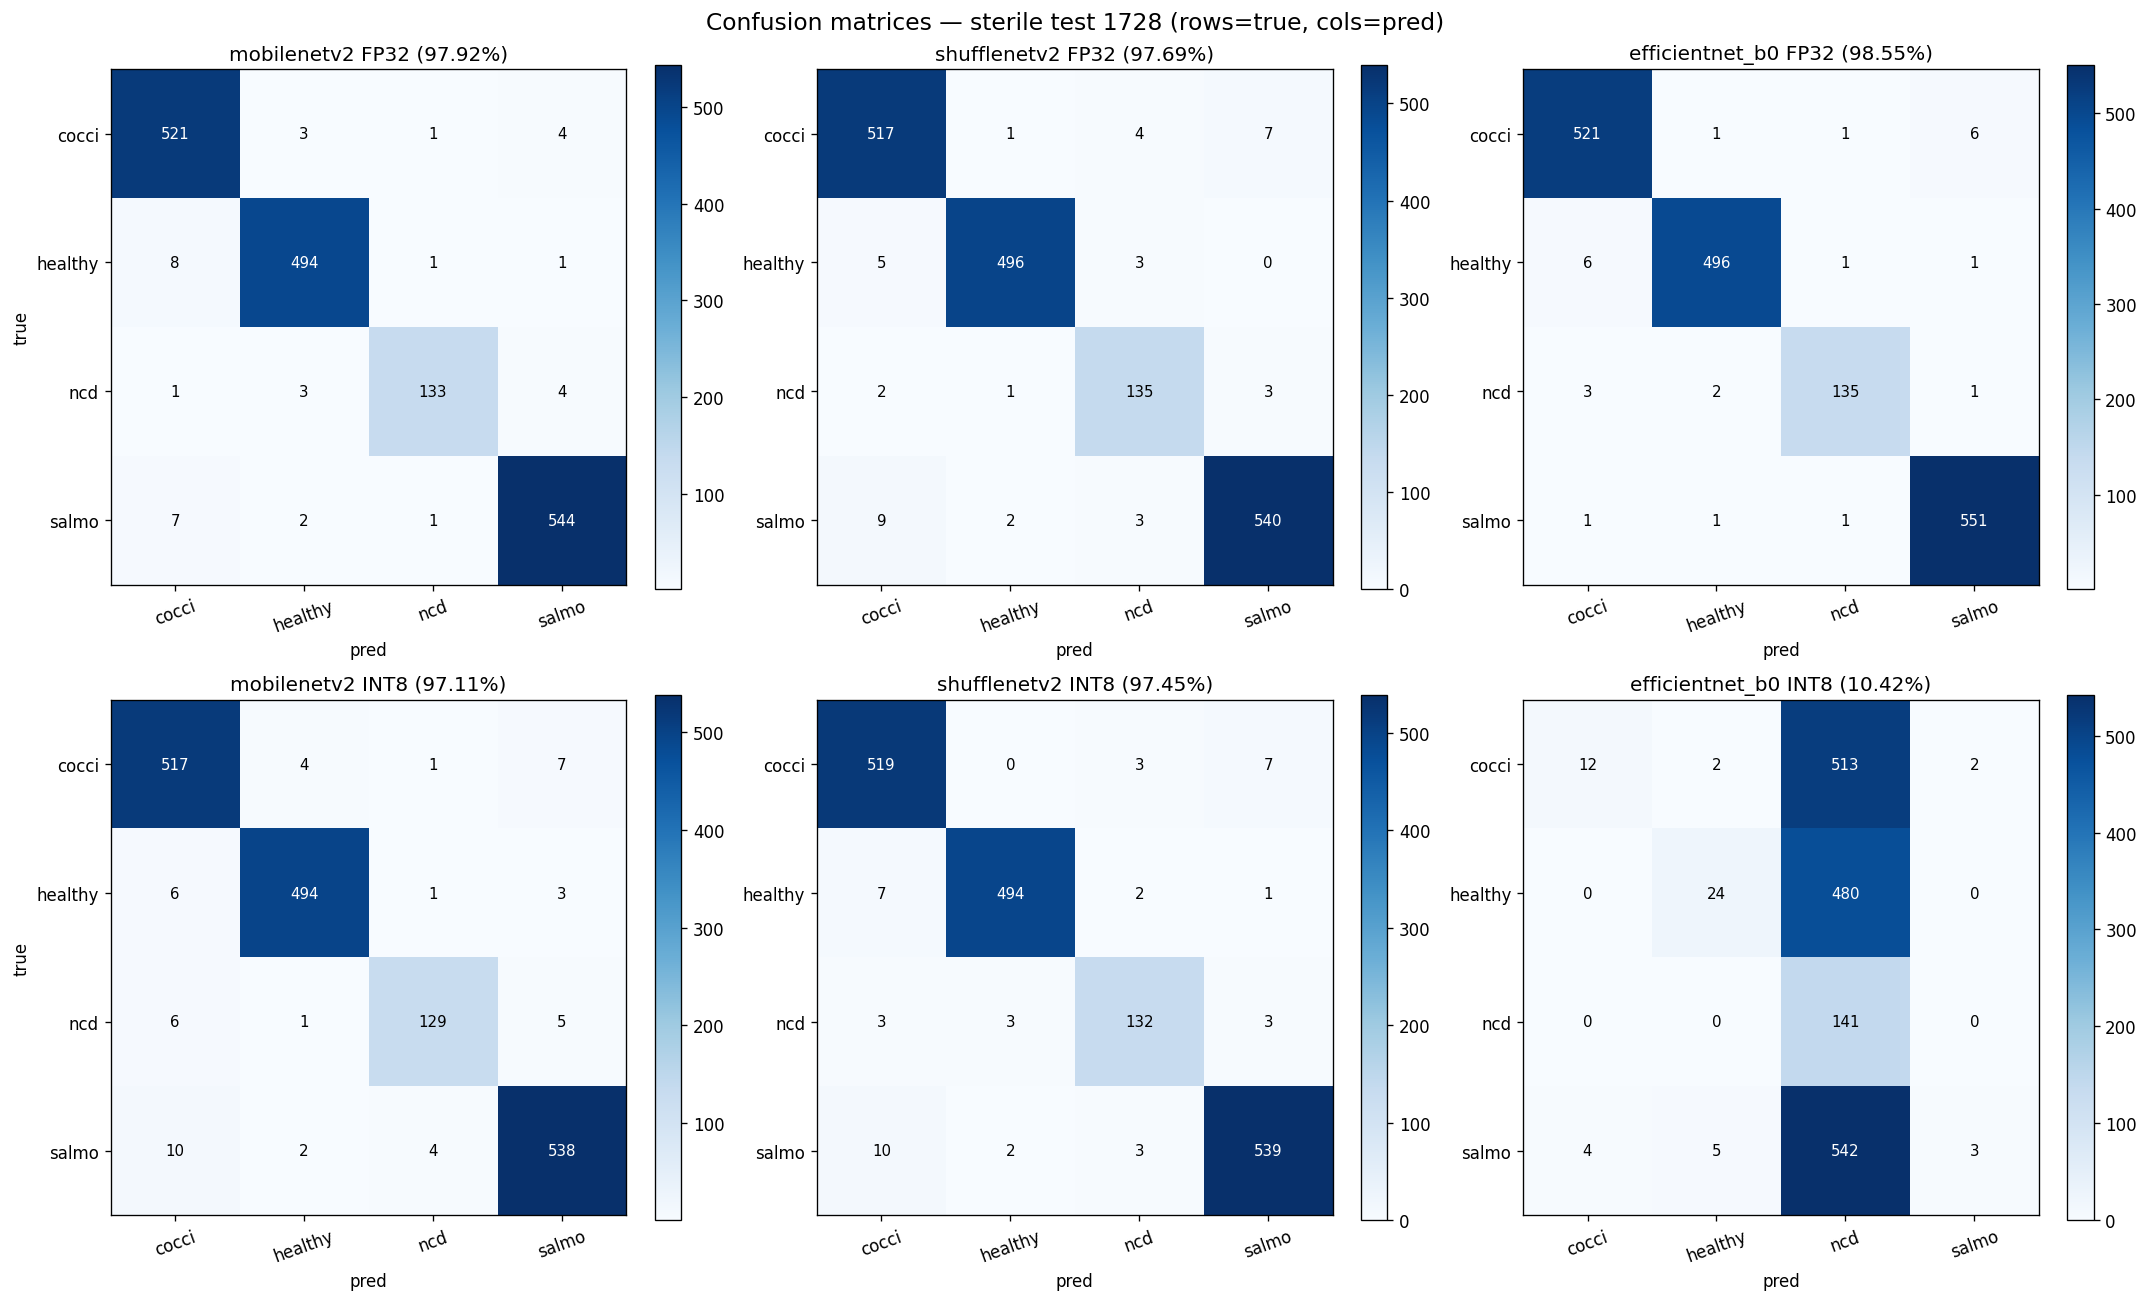
\includegraphics[width=0.95\linewidth]{confusion_gate0.png}
\caption{Confusion matrices on the sterile test set (1,728 images). Top: FP32; bottom: INT8 dynamic. EfficientNet-B0 INT8 (bottom right) collapses to the Newcastle Disease column.}
\label{fig:cm}
\end{figure}

\subsection{Quantization Impact}

Table~\ref{tab:quantization} presents the quantization analysis on the sterile split. All architectures achieve 3.3--3.7$\times$ model size reduction through INT8 quantization.

\begin{table}[htbp]
\caption{INT8 Quantization Analysis (WSL x86 reference, 200 runs). Sterile-split models.}
\label{tab:quantization}
\centering
\begin{tabular}{lccccc}
\toprule
\multirow{2}{*}{Model} & \multicolumn{2}{c}{Size (MB)} & \multicolumn{2}{c}{Latency (ms)} & \multirow{2}{*}{Slowdown} \\
 & FP32 & INT8 & FP32 & INT8 & \\
\midrule
MobileNetV2 & 8.48 & 2.30 & 2.40 & 40.25 & 16.8$\times$ \\
ShuffleNetV2 & 4.89 & \textbf{1.47} & 4.15 & 12.62 & 3.0$\times$ \\
EfficientNet-B0 & 15.3 & 4.16 & 4.35 & 57.18 & 13.1$\times$ \\
\bottomrule
\end{tabular}
\end{table}

INT8 quantization increases latency by 3.0--16.8$\times$ versus FP32 on the x86 reference. Because our reference CPU exposes AVX-VNNI yet still slows down, the bottleneck is the ORT CPU kernel path (dequantize before matmul), not raw ISA absence; Section~IV-C quantifies this overhead on both x86 and ARM.

ShuffleNetV2 degrades least (3.0$\times$ versus 16.8$\times$ for MobileNetV2). Channel-shuffle ops are non-parametric and less sensitive to precision, while MobileNetV2 depthwise separable convolutions are more sensitive.

\subsection{Raspberry Pi~5 Characterization: Thread Scaling and the INT8 Bottleneck}
Table~\ref{tab:rpi5} summarizes sterile-model RPi5 latency at batch=1. FP32 scales with threads: MobileNetV2 drops from 33.16\,ms (1 thread, 30.2\,FPS) to 14.23\,ms (4 threads, 70.3\,FPS, 2.33$\times$ speedup); ShuffleNetV2 from 14.19\,ms to 6.19\,ms (2.29$\times$, 161.5\,FPS); EfficientNet-B0 from 69.45\,ms to 31.56\,ms (2.20$\times$). The sweep covers threads 1 and 4; intermediate thread counts are not measured for the sterile models.

\begin{table}[htbp]
\caption{Raspberry Pi~5 Latency, batch=1 (mean of 200 runs, P50 in parentheses). Sterile-split models, ORT 1.29.0, 44--56$^{\circ}$C, throttled=0x0.}
\label{tab:rpi5}
\centering
\footnotesize
\setlength{\tabcolsep}{3.2pt}
\resizebox{\linewidth}{!}{\begin{tabular}{lccccc}
\toprule
Model & Quant & t=1 & t=4 & Scaling & FP32$\to$INT8 \\
 & & (ms) & (ms) & 1$\to$4 & t=4 \\
\midrule
MobileNetV2 & FP32 & 33.16 (33.00) & \textbf{14.23} (14.03) & 2.33$\times$ & --- \\
 & INT8 & 43.88 (43.86) & 39.83 (39.73) & 1.10$\times$ & 2.80$\times$ slower \\
ShuffleNetV2 & FP32 & 14.19 (14.19) & \textbf{6.19} (6.18) & 2.29$\times$ & --- \\
 & INT8 & 13.65 (13.64) & 11.95 (11.76) & 1.14$\times$ & 1.93$\times$ slower \\
EfficientNet-B0 & FP32 & 69.45 (69.42) & \textbf{31.56} (31.18) & 2.20$\times$ & --- \\
 & INT8 & 76.68 (76.67) & 64.39 (64.19) & 1.19$\times$ & 2.04$\times$ slower \\
\bottomrule
\end{tabular}}
\end{table}

INT8 on RPi5 is slower than FP32 at 4 threads (1.93--2.80$\times$), and its thread scaling stalls: from 1$\rightarrow$4 threads MobileNetV2 INT8 improves only 1.10$\times$ (43.88$\rightarrow$39.83\,ms), ShuffleNetV2 1.14$\times$, EfficientNet-B0 1.19$\times$, versus 2.20--2.33$\times$ for FP32. This indicates limited parallelization of INT8 kernels in ONNX Runtime 1.29.0 on Cortex-A76. One exception: ShuffleNetV2 INT8 at 1 thread (13.65\,ms) is slightly faster than its FP32 counterpart (14.19\,ms), the only configuration where INT8 wins---consistent with its homogeneous channel-shuffle design and lowest node expansion (1.37$\times$).

\begin{figure}[htbp]
\centering
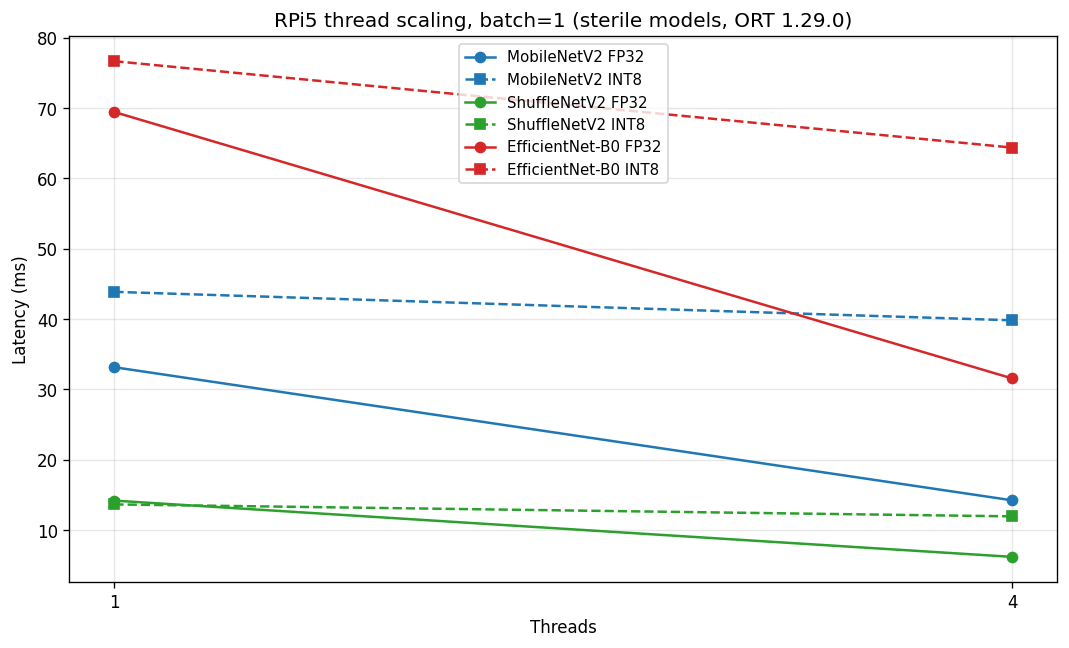
\includegraphics[width=0.95\linewidth]{rpi5_thread_scaling_gate0.png}
\caption{RPi5 thread scaling at batch=1 (sterile models). FP32 (solid) scales from 1 to 4 threads; INT8 (dashed) is flat and slower than FP32 at 4 threads, except ShuffleNetV2 at 1 thread where INT8 is slightly faster.}
\label{fig:rpi5thread}
\end{figure}

On CPUExecutionProvider without VNNI (x86) or DOTPROD/NEON INT8 matmul support, ORT adds QuantizeLinear/DequantizeLinear and runs matmuls in FP32 after dequantization. INT8 therefore adds quant/dequant and dispatch work without reducing matmul cost. Cost grows with the number of quantize boundaries: depthwise separable blocks (MobileNetV2) create many small matmuls and slow down most on x86 (16.8$\times$), while homogeneous channel-shuffle blocks (ShuffleNetV2) slow down least (3.0$\times$). On RPi5 at 4 threads the ranking compresses (2.80/2.04/1.93$\times$). Node expansion measured on the sterile ONNX graphs matches: MobileNetV2 170$\rightarrow$487 (2.86$\times$), EfficientNet-B0 239$\rightarrow$730 (3.05$\times$), ShuffleNetV2 902$\rightarrow$1240 (1.37$\times$). Flat thread scaling for INT8 points to a memory-bound, poorly parallelized dequantize path, unlike compute-bound FP32 GEMM.

Model file size shrinks 3.3--3.7$\times$ with INT8 (e.g., 8.48$\rightarrow$2.30\,MB for MobileNetV2). On the sterile RPi5 sweep (batch=1 only), runtime RSS is similar across quantizations for MobileNetV2 ($\sim$99--108\,MB) and ShuffleNetV2 ($\sim$111--112\,MB), so INT8 does not save RAM at inference on this stack---a practical caveat for memory claims. We do not claim batch-scaling behavior for the sterile models; only batch=1 was measured.

\begin{table}[htbp]
\caption{Level-2 Provenance: Node Expansion on sterile ONNX graphs (dynamic PTQ expands to DynamicQuantizeLinear + ConvInteger + Mul pattern, no static Q/DQ nodes) with ORT kernel quant overhead from RPi5 profiling (10 runs, batch=1, 1 thread). Overhead correlates with expansion and slowdown.}
\label{tab:level2}
\centering
\footnotesize
\setlength{\tabcolsep}{3.0pt}
\resizebox{\linewidth}{!}{\begin{tabular}{lcccccc}
\toprule
Model & FP32 nodes & INT8 nodes & Expansion & DynQuant/CvInt & Quant overhead & x86 / RPi5 slowdown \\
\midrule
MobileNetV2 & 170 & 487 & 2.86$\times$ & 53 / 52 & 29.2\% & 16.8$\times$ / 2.80$\times$ \\
ShuffleNetV2 & 902 & 1240 & 1.37$\times$ & 54 / 56 & 20.7\% & 3.0$\times$ / 1.93$\times$ \\
EfficientNet-B0 & 239 & 730 & 3.05$\times$ & 82 / 81 & 24.9\% & 13.1$\times$ / 2.04$\times$ \\
\bottomrule
\end{tabular}}
\end{table}

\textbf{Measured bottleneck (Level-2).} Table~\ref{tab:level2} quantifies why INT8 is slower. Dynamic PTQ does not insert static QuantizeLinear/DequantizeLinear nodes; it expands each Conv (52--81) into a DynamicQuantizeLinear + ConvInteger + Mul (scale) + Cast pattern, so node count grows by 1.37--3.05$\times$ on the sterile graphs. ORT kernel profiling on RPi5 (batch=1, 1 thread, 10 runs) shows \texttt{Conv\_quant\_kernel} alone consumes 49.5--55.1\% of total time, and all quant-related kernels (QuantizeLinear, scale Mul, Cast, bias-add) add 20.7--29.2\% overhead, while the final \texttt{Gemm\_MatMul\_quant} is $<0.1\%$. The ranking matches the slowdown ranking: MobileNetV2 (29.2\% overhead, 2.86$\times$ expansion) suffers most on x86, ShuffleNetV2 (20.7\%, 1.37$\times$) least. Artifact \texttt{level2\_profiling\_artifact.json} contains per-operator $\mu$s and full op counts (reproducible), complementing TinyML system studies~\cite{david2021}.

\subsection{Accuracy-Latency Tradeoff}

\begin{figure}[htbp]
\centering
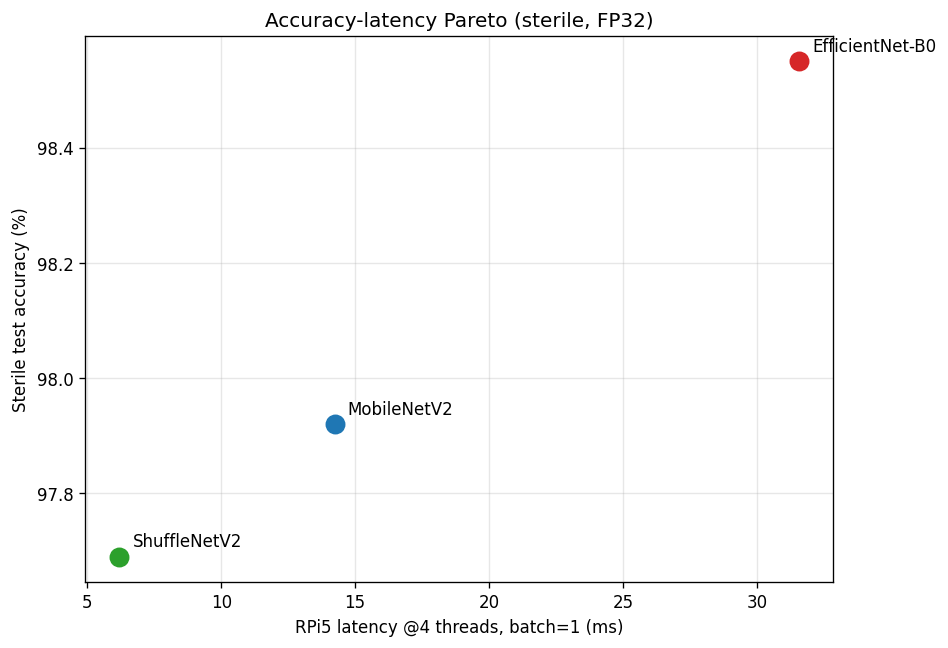
\includegraphics[width=0.95\linewidth]{pareto_gate0.png}
\caption{Accuracy-latency tradeoff (sterile split, FP32). ShuffleNetV2 is fastest (6.19\,ms RPi5 @4 threads, 97.69\%); EfficientNet-B0 is most accurate (98.55\%) at 31.56\,ms; MobileNetV2 is balanced (97.92\%, 14.23\,ms).}
\label{fig:pareto}
\end{figure}

The accuracy-latency plot (Fig.~\ref{fig:pareto}) shows that the fastest model is ShuffleNetV2 FP32 at 6.19\,ms RPi5 (161.5\,FPS), the most accurate is EfficientNet-B0 FP32 at 98.55\%, and MobileNetV2 FP32 is the balanced middle (97.92\%, 14.23\,ms). The gap between best and worst FP32 accuracy is only 0.86pp (97.69\% versus 98.55\%); hardware constraints and quantization scheme should drive model choice for deployment.

\begin{figure}[htbp]
\centering
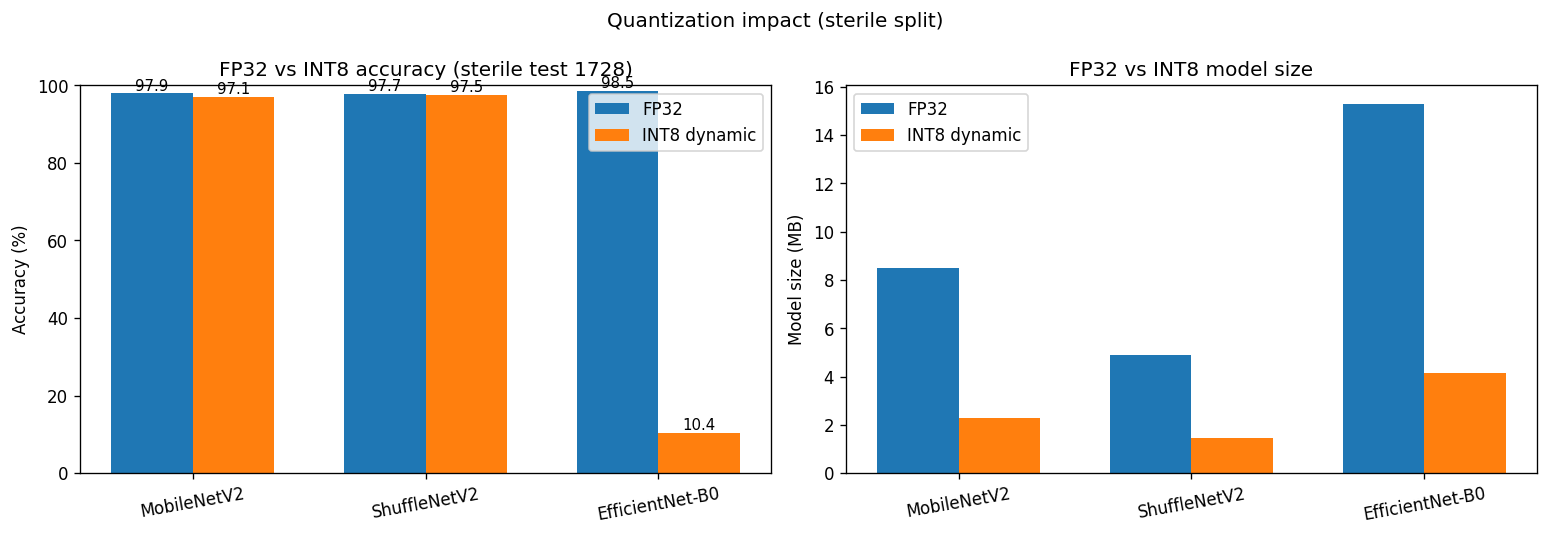
\includegraphics[width=0.95\linewidth]{quant_acc_size_gate0.png}
\caption{Quantization impact on the sterile split: accuracy is preserved for MobileNetV2 and ShuffleNetV2 but collapses for EfficientNet-B0 under dynamic INT8, while model size shrinks 3.3--3.7$\times$ for all three.}
\label{fig:quantimpact}
\end{figure}

\subsection{Grad-CAM Interpretability}

\begin{figure}[htbp]
\centering
\includegraphics[width=0.95\linewidth]{gradcam_mobilenetv2.png}
\caption{Grad-CAM visualization for MobileNetV2 across four fecal disease classes. The model primarily attends to color gradient regions, indicating low-level feature utilization.}
\label{fig:gradcam}
\end{figure}

Grad-CAM analysis~\cite{selvaraju2017} (Fig.~\ref{fig:gradcam}) provides a descriptive attention map for MobileNetV2: attention concentrates on color gradient regions, consistent with depthwise convolutions capturing local texture. We show a single MobileNetV2 map as illustration only and make no cross-architecture attention claims; quantization sensitivity is diagnosed via the per-tensor vs per-channel experiment above.

\subsection{Comparison with Related Work}

\begin{table}[htbp]
\caption{Comparison with Existing Work}
\label{tab:comparison}
\centering
\begin{tabular}{lcccc}
\toprule
Work & Dataset & Best & Acc. & Edge \\
 & & Model & (\%) & Analysis \\
\midrule
Dhungana~\textit{et al.}~\cite{dhungana2025} & Machuve & EB0 & 99.1 & Web \\
Tasdelen~\textit{et al.}~\cite{tasdelen2025} & Machuve & MN2 & 97.1 & --- \\
Degu~\textit{et al.}~\cite{degu2023} & Machuve & R50 & 98.7 & Mobile \\
\textbf{Ours} & \textbf{Machuve} & \textbf{EB0} & \textbf{98.6} & \textbf{+INT8+diagnosis} \\
\bottomrule
\end{tabular}
\end{table}

Our accuracy (98.55\%) is competitive with prior results on the same dataset while providing additional analysis in quantization diagnosis, tradeoff characterization, and interpretability that are absent from prior work.

\section{Conclusion}

This paper characterizes lightweight CNN architectures with INT8 quantization for poultry fecal disease detection. Our key findings are:

All three architectures exceed 97\% FP32 accuracy with ImageNet transfer learning on the sterile split, with EfficientNet-B0 at 98.55\%. Dynamic INT8 PTQ preserves MobileNetV2 (97.11\%) and ShuffleNetV2 (97.45\%) but collapses EfficientNet-B0 to 10.42\%; static per-channel quantization recovers EfficientNet-B0 to 94.56\%, localizing the failure to per-tensor depthwise quantization. On x86 reference hardware, INT8 increases latency by 3.0--16.8$\times$ (ShuffleNetV2 least, MobileNetV2 most); on RPi5 INT8 is 1.9--2.8$\times$ slower at 4 threads and scales by only 1.10--1.19$\times$ from 1 to 4 threads versus 2.20--2.33$\times$ for FP32. ShuffleNetV2 degrades least (3.0$\times$ on x86, 1.93$\times$ on RPi5) due to its homogeneous design; notably ShuffleNetV2 INT8 at 1 thread is the only configuration faster than its FP32 counterpart (13.65 vs 14.19\,ms). On RPi5, batch 1 is the measured operating point and INT8 size reduction (3.3--3.7$\times$) does not reduce runtime RSS. The tradeoff analysis identifies ShuffleNetV2 FP32 for the lowest RPi5 latency (6.19\,ms at 4 threads) and MobileNetV2 FP32 as balanced (14.23\,ms, 97.92\%).

These findings enable practitioners to make informed deployment decisions based on their specific hardware constraints. This work characterized RPi5 deployment; future work includes QAT comparison against the PTQ diagnosis here, energy measurement on RPi5, and class imbalance mitigation for the underrepresented NCD class.

Code and sterile-split artifacts (dedup audit, split manifests, eval JSONs, benchmark logs, plotting scripts) are available at \url{https://github.com/jaweed3/paper_poultry_p2/tree/post30-gate0-dedup}.

\begin{thebibliography}{99}

\bibitem{dhungana2025}
A.~Dhungana, X.~Yang, B.~Paneru, S.~Dahal, G.~Lu, and L.~Chai, ``An integrated deep learning approach for poultry disease detection and classification based on analysis of chicken manure images,'' \emph{AgriEngineering}, vol.~7, no.~9, p.~278, 2025. DOI: 10.3390/agriengineering7090278.

\bibitem{machuve2022}
D.~Machuve \textit{et al.}, ``Poultry diseases diagnostics models using deep learning,'' \emph{Frontiers in Artificial Intelligence}, vol.~5, p.~733345, 2022. DOI: 10.3389/frai.2022.733345.

\bibitem{tasdelen2025}
A.~Tasdelen and Y.~Arslan, ``Detection of high-risk diseases in poultry feces through transfer learning,'' \emph{Engineering Science and Technology, an International Journal}, vol.~64, p.~102002, 2025. DOI: 10.1016/j.jestch.2025.102002.

\bibitem{degu2023}
M.~Z.~Degu and G.~L.~Simegn, ``Smartphone based detection and classification of poultry diseases from chicken fecal images using deep learning techniques,'' \emph{Smart Agricultural Technology}, vol.~4, p.~100221, 2023. DOI: 10.1016/j.atech.2023.100221.

\bibitem{mobilenetv2}
M.~Sandler, A.~Howard, M.~Zhu, A.~Zhmoginov, and L.-C.~Chen, ``MobileNetV2: Inverted residuals and linear bottlenecks,'' in \emph{Proc. IEEE CVPR}, 2018, pp.~4510--4520.

\bibitem{shufflenetv2}
N.~Ma, X.~Zhang, H.-T.~Huang, and J.~Sun, ``ShuffleNetV2: Practical guidelines for efficient CNN architecture design,'' in \emph{Proc. ECCV}, 2018, pp.~116--131.

\bibitem{efficientnet}
M.~Tan and Q.~V.~Le, ``EfficientNet: Rethinking model scaling for convolutional neural networks,'' in \emph{Proc. ICML}, 2019, pp.~6105--6114.

\bibitem{jacob2018}
B.~Jacob \textit{et al.}, ``Quantization and training of neural networks for efficient integer-arithmetic-only inference,'' in \emph{Proc. IEEE CVPR}, 2018, pp.~2704--2713.

\bibitem{chi2026}
T.-Y.~Chi, ``FecalFed: Privacy-preserving poultry disease detection via federated learning,'' \textit{arXiv:2604.00559}, 2026.

\bibitem{usda2024}
U.S.~Department of Agriculture, National Agricultural Statistics Service, ``Poultry production and value: 2023 summary,'' Apr. 2024. [Online]. Available: \url{https://www.nass.usda.gov/Publications/Todays_Reports/reports/plyaan24.pdf}

\bibitem{hoang2026}
T.-M.~Hoang \textit{et al.}, ``A comprehensive evaluation of lightweight deep learning models for tomato disease classification on edge computing environments,'' \emph{Scientific Reports}, vol.~16, p.~12320, 2026. DOI: 10.1038/s41598-026-42439-6.

\bibitem{onnxruntime2024}
Microsoft, ``Quantize ONNX models,'' ONNX Runtime Documentation, 2024. [Online]. Available: \url{https://onnxruntime.ai/docs/performance/quantization.html}

\bibitem{machuve22}
D.~Machuve \textit{et al.}, ``Machine learning dataset for poultry diseases diagnostics,'' Zenodo, 2022. DOI: 10.5281/zenodo.4628934.

\bibitem{nagel2021}
M.~Nagel \textit{et al.}, ``A white paper on neural network quantization,'' \textit{arXiv:2106.08295}, 2021.

\bibitem{selvaraju2017}
R.~R.~Selvaraju \textit{et al.}, ``Grad-CAM: Visual explanations from deep networks via gradient-based localization,'' in \emph{Proc. IEEE Int. Conf. Comput. Vis. (ICCV)}, 2017, pp.~618--626.

\bibitem{deng2009}
J.~Deng \textit{et al.}, ``ImageNet: A large-scale hierarchical image database,'' in \emph{Proc. IEEE Conf. Comput. Vis. Pattern Recognit. (CVPR)}, 2009, pp.~248--255.

\bibitem{david2021}
R.~David \textit{et al.}, ``TensorFlow Lite Micro: Embedded machine learning for TinyML systems,'' in \textit{Proc. Machine Learning and Systems (MLSys)}, 2021, pp.~800--815.

\end{thebibliography}

\end{document}
